\documentclass[11pt,a4paper]{article}

\usepackage[applemac]{inputenc}
\usepackage{latexsym}
\usepackage{graphicx}
\usepackage[english]{babel}


\usepackage{amsmath,amssymb}
\usepackage{pstricks,pst-plot}
\usepackage{calc}
\usepackage{multicol}
\usepackage{fancyhdr}
\usepackage{lastpage}
\usepackage[T1]{fontenc}
\usepackage{lmodern}
\usepackage{stmaryrd}
\usepackage[]{algorithm2e}
\usepackage{float}
\usepackage{fullpage}
\usepackage{ bbold }% indicator function

\pagestyle{plain}



\begin{document}

\title{Kernel Methods HW2 : Implementation}
\author{Mathurin \textsc{Massias} \and Clement \textsc{Nicolle}}
\date{\today} 

\maketitle

\hspace{-6mm}

We worked with Python 2.7.
\\A point in the dataset is in dimension 257 : the digit id (0 to 9) and the 256 gray scale values of the $16 \times 16$ pixels of the image. We remove the digit id as we are not doing classification here.

\begin{figure}[H]
	\centering
	\noindent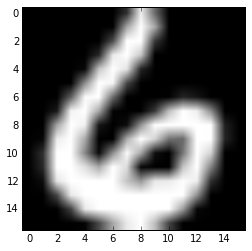
\includegraphics[scale=0.4]{six.png}
	\caption{Example of an image in the dataset, a six here}
\end{figure}

We projected 200 points on the first two principal components using linear, polynomial and Gaussian kernel :
\begin{figure}[H]
	\centering
	\noindent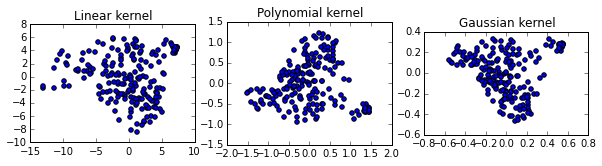
\includegraphics[scale=0.7]{kpca.png}
	\caption{Results of KPCA on the first two dimensions for different kernels}
\end{figure}

We now add a Gaussian noise to the image, and will aim to remove it :
\begin{figure}[H]
	\centering
	\noindent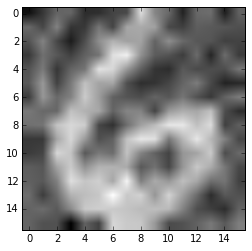
\includegraphics[scale=0.7]{noisy.png}
	\caption{Noisy image}
\end{figure}

The proposed method consists in finding the image from the original dataset which is the closest to the projection of our noisy image on the first $d$ kernel principal components of the dataset. It is done using a gradient descent iterative algorithm.

\end{document}